\documentclass{article}

\usepackage{hyperref}
\usepackage{listings}
\usepackage{amsmath}

\usepackage{tikz}
\usetikzlibrary{matrix,positioning,arrows.meta,arrows}

\RequirePackage{color}
\definecolor{codegreen}{rgb}{0,0.6,0}
\definecolor{codegray}{rgb}{0.5,0.5,0.5}
\definecolor{codepurple}{rgb}{0.58,0,0.82}
\definecolor{backcolour}{rgb}{0.95,0.95,0.92}

\lstdefinestyle{python}{
    language = Python,
    commentstyle=\color{codegreen},
    keywordstyle=\color{blue},
    numberstyle=\tiny\color{codegray},
    stringstyle=\color{codepurple},
    breakatwhitespace=false,
    breaklines=true,
    captionpos=b,
    keepspaces=true,
    showspaces=false,
    showstringspaces=false,
    showtabs=false,
    backgroundcolor=\color{backcolour},
    tabsize=2
}
\lstset{style = Python}

\usepackage{natbib}
\bibliographystyle{plainnat}

\begin{document}

\section{Introduction}

Segyio is a fast library with a powerful Python interface for reading and
writing seismic data in SEG-Y format, and is licenced under the LGPL
\citep{lgplv3}. More than 40 years have passed since the first revision of
SEG-Y \citep{barry}, and many commercial and free products have the capability
to read and write this format. This feature is often a loader or writer
component inside a larger application or suite for seismic processing.

In contrast to the large geophysics suites, with transformations,
visualisations, pre-written mathematics and workflow management, segyio is a
small and embeddable library. Really, the only thing segyio does is provide
features for reading and manipulating SEG-Y files. This means segyio is well
suited to power SEG-Y support in new applications, such as handling wavefield
data for a machine learning system. Because segyio is a \emph{library}, it is a
powerful tool for experimentation and innovation: it enables the scientist to
inspect and plot arbitrary data, and develop new machine learning models,
visualisations and new geophysical models, without having to worry about
details and intricacies of SEG-Y. In Equinor we have several programs and
workflows with SEG-Y support powered by segyio, and segyio also drives the I/O
facilities of the Malenov \citep{malenov} machine learning tool.

The segyio source code is available at \url{https://github.com/equinor/segyio}

\section{Design and method}

Segyio is designed from the ground-up assuming that:
\begin{itemize}
    \item Segyio should look and feel like Python
    \item Segyio should quickly get out of the way
    \item Fast random traces to individual traces is useful
    \item Simple and \emph{pythonic} code should be reasonably performant
\end{itemize}

The first point is adressed by carefully designing interfaces that with syntax
similar to the popular numpy \citep{numpy} library. SEG-Y files come with
varying levels of structure, which segyio tries to detect and make available to
users.  The basic abstraction, the \emph{trace}, pretends that the SEG-Y file
is a large array in memory, when in fact every trace is read from disk on
request.

\begin{figure}[h]
    \resizebox{\textwidth}{!}{
        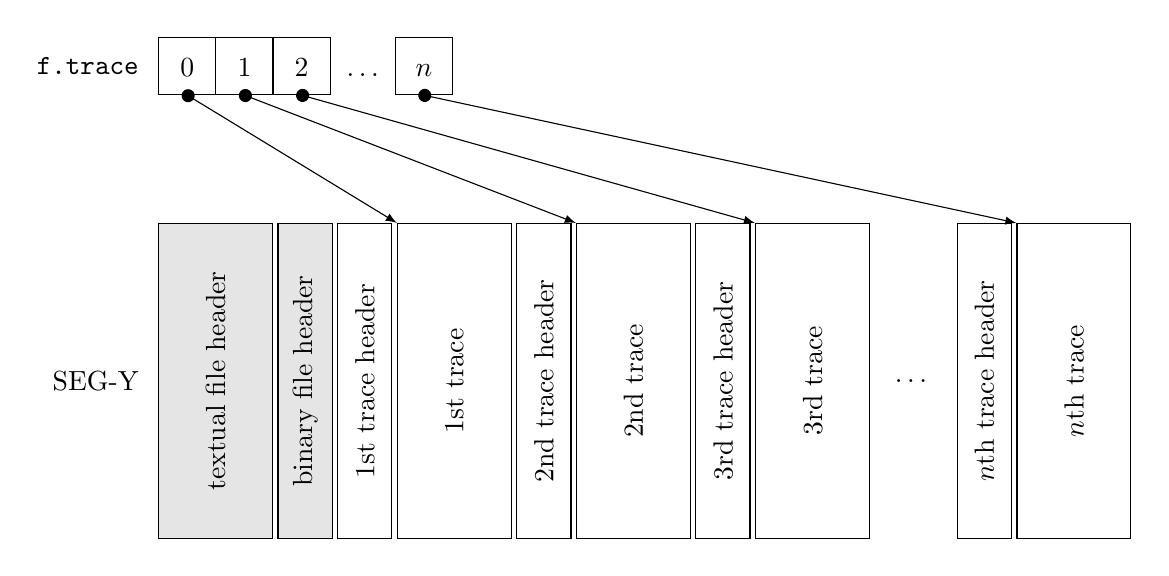
\begin{tikzpicture}[>=latex]
\tikzset{
mymat/.style={
  matrix of math nodes,
  text height=2.5ex,
  text depth=0.75ex,
  text width=3.25ex,
  align=center,
  column sep=-\pgflinewidth,
  style={nodes=draw}
  },
mymats/.style={
  matrix,
  align=center,
  style={nodes={draw, minimum height=4cm}},
  column sep=4\pgflinewidth
  }
}

\matrix [mymat, anchor=west] at (0,0)
(ftrace)
{
    0 & 1 & 2 & \node[draw=none, text width=4ex] {\dots}; & n \\
};
\matrix [mymats, anchor=west] at (0,-4)
(segy)
{
    \node [fill=gray!20, text width=8ex] {\rotatebox{90}{textual file header}}; &
    \node [fill=gray!20, text width=3ex] {\rotatebox{90}{binary file header}};  &
    \node (h1) [text width=3ex]          {\rotatebox{90}{1st trace header}}; &
    \node (t1) [text width=8ex]          {\rotatebox{90}{1st trace}}; &
    \node (h2) [text width=3ex]          {\rotatebox{90}{2nd trace header}}; &
    \node (t2) [text width=8ex]          {\rotatebox{90}{2nd trace}}; &
    \node (h3) [text width=3ex]          {\rotatebox{90}{3rd trace header}}; &
    \node (t3) [text width=8ex]          {\rotatebox{90}{3rd trace}}; &
    \node [draw=none, text width=5ex]    {$\dots$}; &
    \node (hn) [text width=3ex]          {\rotatebox{90}{$n$th trace header}}; &
    \node (tn) [text width=8ex]          {\rotatebox{90}{$n$th trace}}; \\
};

\node[left=0pt of ftrace](ftracelabel) {\verb|f.trace|};
\node[left=0pt of segy](filelabel) {SEG-Y};

\begin{scope}[shorten <= -2pt]
    \draw[*->] (ftrace-1-1.south) to[looseness=0, out=-90] (t1.north west);
    \draw[*->] (ftrace-1-2.south) to[looseness=0, out=-90] (t2.north west);
    \draw[*->] (ftrace-1-3.south) to[looseness=0, out=-90] (t3.north west);
    \draw[*->] (ftrace-1-5.south) to[looseness=0, out=-90] (tn.north west);
\end{scope}

\end{tikzpicture}

    }
    \caption{Traces as a virtual array}
\end{figure}

Reading traces on-demand means segyio can handle files much larger than the
available memory, without any user intervention. Other common array operations,
such as slicing, are also available. In addition to an array interface, segyio
supports inline and crossline access and pre-stack volumes. Segyio can read the
text, trace, and binary headers, and provides some other useful tools, common
operations such as the \verb|cube| function for reading a 3D volume from SEG-Y
into a 3D numpy array.

Segyio uses the numpy \verb|ndarray| as the primary data type for returning
data to users, which means that sophisticatedand fast numerics can be
immediately applied to data from virtually all of segyio's function calls. This
small detail give users a lot of flexibility and power.

SEG-Y is an old standard, designed for very different computers than our modern
laptops, desktops, and clusters. A lot of SEG-Y files still use IBM float,
which segyio handles and transforms to a native (usually IEEE 754)
representation under the hood. SEG-Y is also designed with magnetic tape in
mind as the primary storage medium. Magnetic tape behaves very differently from
modern storage media, in particular because tape can only be read linearly,
\emph{not} randomly. To read a trace in the middle of a SEG-Y file on tape, the
tape reader would have to physically wind through the tape from the front to
the right location in the tape roll. Modern hard- and solid state drives can
seek to arbitrary locations in virtually constant time.

In segyio, random access to traces is achieved by assuming all traces are of
equal length. The SEG-Y standard explicitly allows for traces to vary in
length, but in practice this does not happen often. With this assumption,
by knowing the number of traces, the position of every individual trace can be
computed, and segyio can quickly read any trace.

To make simple code performant, segyio encourages and supports use of python
\emph{protocols}. In Python, protocols are interfaces that specific syntax
relies on, such as the \verb|iter| and \verb|next| functions. Python
programmers rarely use these functions directly, but they are the drivers
powering the \verb|for| loop and, more generally, iteration. Code written using
these protocols is referred to in the Python community as \emph{pythonic}. When
these standard protocols are used with segyio objects, some optimisations are
done such scheduling more work to the C library, or by reusing a single array
allocation.

\section{Building programs with segyio}

Segyio offers no functionality for working with the actual data - instead,
segyio attempts to be a useful building block in larger programs, where reading
and writing SEG-Y files is just a small, and arguably uninteresting, detail.

Consider this simple program to calculate the sample-wise difference between
two files (left and right), and write the difference to a third file (out):

\begin{minipage}{\linewidth}
\begin{lstlisting}
with segyio.open(fin1) as left, segyio.open(fin2) as right:
    with segyio.open(fout, mode = 'r+') as out:
        for i in range(len(left.trace)):
            out.trace[i] = left.trace[i] - right.trace[i]
\end{lstlisting}
\end{minipage}

The subtraction operator \verb|-| is numpy's element-wise subtraction, because
\verb|left[i]| and \verb|right[i]| read from the files into numpy arrays.

Segyio strives to make simple and elegant code fast. To achieve this, segyio
implements support for the \emph{iterator} \citep{pep-iterator} protocol. The
following two snippets are functionally equivalent, but the first version is
faster.

\begin{minipage}{\linewidth}
\begin{lstlisting}
# using the iterator protocol and non-indexed access
for trace in left.trace:
    if numpy.any(numpy.where(trace < 0)):
        print('Trace with negative value')

# using range(...) and trace indices
for i in range(len(left.trace)):
    if numpy.any(numpy.where(left.trace[i] < 0)):
        print('Trace with negative value')
\end{lstlisting}
\end{minipage}

In- and crosslines are accessed with a similar interface, and work analogous to
these examples.

\section{Conclusion}

Segyio is a small library that can provide SEG-Y support for new machine
learning systems, applications and utilities for seismic processing. It
integrates with Python protocols and idioms to provide a simple, fast, and
intuitive interface, suitable both for interactive use, small tools, and large
applications.

\bibliography{segyio.bib}

\end{document}
